\subsection{Modeling Tools}
\noindent The main tool used for this project is the Medium-Energy Gamma-ray Astronomy library (MEGAlib). MEGAlib is a set of software tools which are designed to simulate and analyze data of gamma-ray detectors, with a specialization on Compton telescopes. While MEGAlib was originally developed for astrophysics, it has been expanded and used for ground based applications such as medical imaging and environmental monitoring. MEGAlib contains a geometry and detector description tool for the detailed modeling of different detector types and characteristics, and provides an easy to use simulation program based on Geant4. Within MEGAlib, the two tools used to simulate the search scenario are Geometry for MEGAlib (Geomega) and the Cosmic Simulator (Cosima). Geomega allows for the creation of precise and unique geometries in which to run simulations \cite{cosima}. Cosima generates particles within the Geomega geometry and provides detailed information on every particle interaction in an output sim file \cite{cosima}. Of interest to this project, the Cosima output provides positional information on the particles interaction in material (scattering) and where it impacted the detector.

\begin{figure}[!htb]
  \centering
  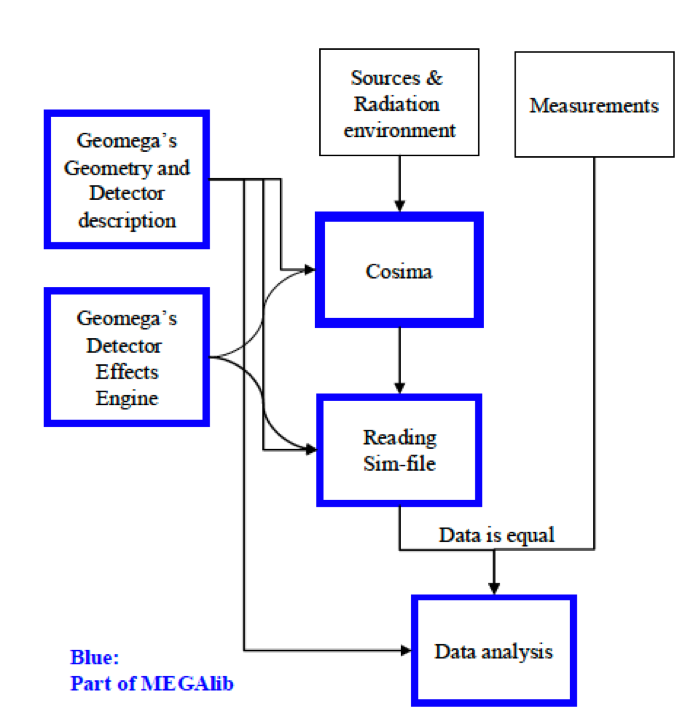
\includegraphics[width=\columnwidth]{images/MEGAlib}
  \caption{Work flow of MEGAlib simulation}
  \label{fig:MEGAlib}
\end{figure}

Fig. \ref{fig:MEGAlib} displays the work flow of a MEGAlib simulation. In addition to MEGAlib, extensive python coding is required to parse the sim file, quantify surface flux, and localize sources.

\subsection{Simulating Camp Roberts}
The intended model is a detector system mounted on a UAS conducting a flight around a target building. In addition to unknown source, activity, and location, the geometry and material composition of the buildings at Camp Roberts are also unknown. Moreover, distance and lack of access made measuring and material sampling an unfeasible option. Instead, a standard three story concreter building on an asphalt slab was modeled using ASTM Building and Construction Standards. Material composition of concrete and asphalt were modeled using the Pacific Northwest National Laboratory Compendium of Material Composition for Radiation Transport Modeling \cite{compendium}. Tables \ref{table:concrete} and \ref{table:asphalt} show the material composition of concrete and asphalt.

\begin{table}[!htp]
 \caption{Material Composition of Concrete}
  \begin{center}
    \begin{tabulary}{\columnwidth}{ccc}
      \hline
      Concrete & 2.3 g/cm$^{3}$\\ \hline
      Element & Weight Fraction\\ \hline
      H & 0.022100  \\
      C & 0.002484 \\
      O & 0.574930 \\
      Na & 0.015208 \\
      Mg & 0.001266 \\
      Al & 0.019953 \\
      Si & 0.304627 \\
      K & 0.010045 \\
      Ca & 0.042951 \\
      Fe & 0.006435 \\ \hline
    \end{tabulary}
  \end{center}
  \label{table:concrete}
\end{table}

\begin{table}[!htp]
 \caption{Material Composition of Asphalt Pavement}
  \begin{center}
    \begin{tabulary}{\columnwidth}{ccc}
      \hline
      Asphalt & 2.5784 g/cm$^{3}$\\ \hline
      Element & Weight Fraction\\ \hline
      H & 0.007781\\
      C & 0.076175\\
      N & 0.000363\\
      O & 0.459103\\
      Na & 0.011659\\
      Mg & 0.021757\\
      Al & 0.051009\\
      Si & 0.231474\\
      S & 0.002804\\
      K & 0.017058\\
      Ca & 0.084471\\
      Ti & 0.003403\\
      V & 0.000024\\
      Mn & 0.000362\\
      Fe & 0.031375\\
      Ni & 0.000002\\
      Pb & 0.001179\\ \hline
    \end{tabulary}
  \end{center}
  \label{table:asphalt}
\end{table}

To ensure the model provided multiple use cases, the first floor was modeled with an open door, the second floor was partitioned into four equally sized rooms, and the top floor was fully enclosed. The exact measurement of the building are 6.2m x 6.2m x 9m, with a wall, roof, and floor thickness of 10 cm. The asphalt slab is 20m x 20m x 0.5m. The flight path of the detector around the building is approximated using a cylindrical blackbody absorber (i.e. every simulated particle will be collected) with a cap around the building. The blackbody absorber has a 10m radius centered on the building and is 14m tall.

\begin{figure}[!htb]
  \centering
  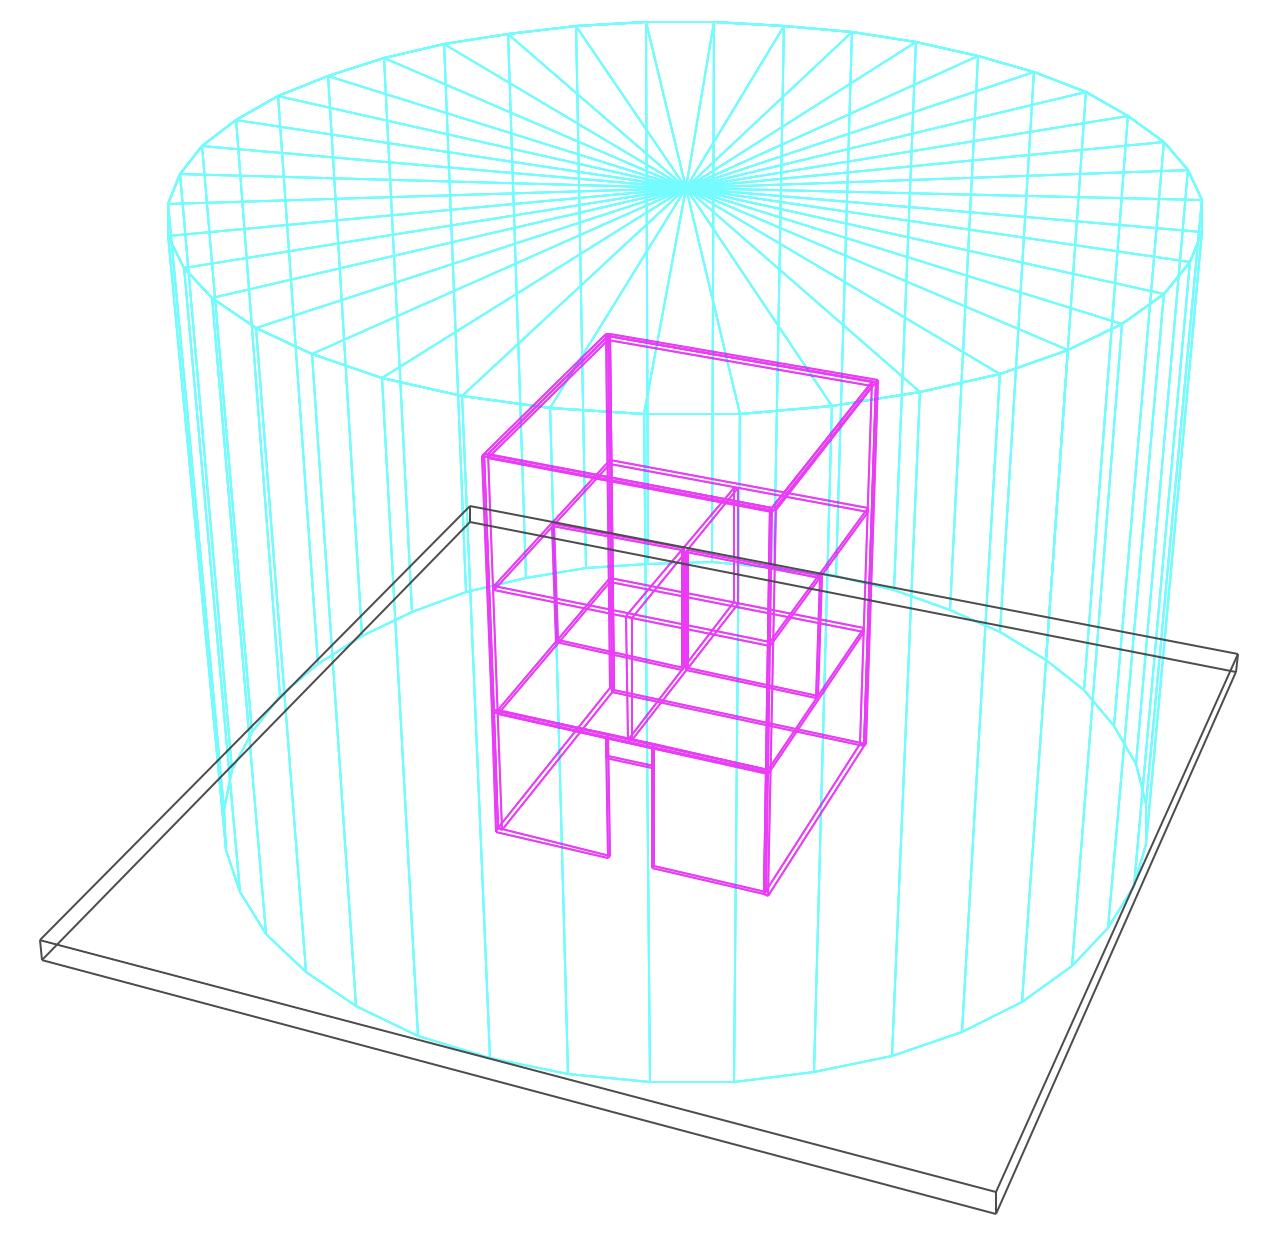
\includegraphics[width=\columnwidth]{images/model}
  \caption{Geomega model of building (pink), slab (black), and detector (cyan)}
  \label{fig:model}
\end{figure}

Fig. \ref{fig:model} displays the simulation geometry. The source was simulated in nine locations (three on each floor) of varying height and distance from detector.

\begin{table}[!htp]
 \caption{Source Locations for Simulations}
  \begin{center}
    \begin{tabulary}{\columnwidth}{ccccc}
      \hline
      Floor & Location & x [cm] & y [cm] & z [cm] \\ \hline
      1 & Central & 50 & -50 & 50 \\
      1 & Middle & 150 & -150 & 150 \\
      1 & Wall & 250 & -250 & 250 \\
      2 & Central & 50 & -50 & 350 \\
      2 & Middle & 150 & -150 & 450 \\
      2 & Wall &250 & -250 & 550 \\
      3 & Central & 50 & -50 & 650 \\
      3 & Middle & 150 & -150 & 750 \\
      3 & Wall & 250 & -250 & 850 \\ \hline
    \end{tabulary}
  \end{center}
  \label{table:positions}
\end{table}

Table \ref{table:positions} shows the simulated source locations. The floor at the center of the building is at (0,0,0).

\subsection{The Inverse Square Law of Radiation}
\label{subsec:inverse}
\noindent The counts registered by a detector is governed by Poisson statistics and decreases inversely with the square of distance. Assuming the source emits radiation isotropically, the count rate in the detector, CR, in s$^{-1}$ can be defined as \cite{morse}:

\begin{align}
CR = \frac{A B A_{d} \eta} {4\pi r^2} \label{eq1}
\end{align}

Where $A$ is the source activity, $B$ is the branching ratio, $A_{d}$ is is the detector area, $\eta$ is the detector efficiency, and $r$ is the distance from the source to the detector. When gammas are transmitted through materials the possibility on interaction with materials is governed by the density of the material, $\rho$, the mass attenuation coefficient for that specific energy, $\mu$/$\rho$, and the attenuation length, $\Delta$$L$.The count rate of full energy deposition in to detector can be defined as \cite{morse}:

\begin{align}
CR = \frac{A B A_{d} \eta e^(\frac{\mu}{\rho}\Delta L)} {4\pi r^2} \label{eq2}
\end{align}
\\\\
Based on the above principle, the detector response in simulations should be highly dependent on the distance of the source from the detector and the amount of attenuation.
